\documentclass[a4paper,10pt]{article}
\usepackage[utf8]{inputenc}
\usepackage[T1]{fontenc}
\usepackage{lmodern}
\usepackage[ngerman]{babel}
\usepackage[a4paper,portrait,left=22mm,right=22mm,top=22mm,bottom=24mm]{geometry}
\usepackage{longtable,array,booktabs}
\usepackage{tabularx}
\usepackage{graphicx}
\usepackage{float}
\usepackage{xcolor}
\usepackage{enumitem}
\usepackage{microtype}
\usepackage{fancyhdr}
\usepackage{amsmath}
\usepackage[font=small,skip=5pt]{caption}
\usepackage{subcaption}
\pagestyle{fancy}
\fancyhf{}
\fancyfoot[L]{\small\texttt{C3\_SPM\_Blatt4.pdf}}
\fancyfoot[R]{\small Seite \thepage}
\renewcommand{\headrulewidth}{0pt}
\renewcommand{\footrulewidth}{0.4pt}
\setlength{\footskip}{22pt}
\setlength{\parindent}{0pt}
\setlength{\parskip}{4pt}
\setlength{\emergencystretch}{3em}
\setlist{nosep,leftmargin=*,topsep=3pt}
\clubpenalty=10000
\widowpenalty=10000
\displaywidowpenalty=10000
\raggedbottom
\setlength{\tabcolsep}{4pt}
\renewcommand{\arraystretch}{1.15}
\newcolumntype{Z}{>{\centering\arraybackslash}X}
\newcolumntype{C}[1]{>{\centering\arraybackslash}p{#1}}
\setlength{\LTpre}{4pt}
\setlength{\LTpost}{8pt}
\setlength{\LTcapwidth}{\textwidth}
\newcommand{\sectionspace}[1]{\par\ifdim
                                      \dimexpr\pagegoal-\pagetotal\relax<#1\relax\newpage
\fi\addvspace{14pt}}
\newcommand{\offen}{\emph{noch offen}}


\title{Projektstand und Prototyp\\{\large Übungsblatt 4}}
\author{Gruppe C3 / MoinMetrics\\{}Alexander Borrmann\\{}Lukas Pancratius\\{}Ino Wölke}
\date{Hochschule Emden-Leer\\Software-Projektmanagement\\Wintersemester 2026/27\\Prof. Dr. Gerrit Jan Veltink\\[1em]Berichtsdatum: 22.11.2026}
\begin{document}
\maketitle
\thispagestyle{fancy}
\clearpage
\section*{Aufgabe 1: Aufwandserfassung}
\subsection*{Plan-Ist-Vergleich}
Die Planaufwände und Bezeichnungen sind aus den Arbeitspaketen von Blatt 3 übernommen und in Personenstunden angegeben. Die Ist-Werte für AP 4 und AP 5 beruhen auf der Aufwandserfassung; der Ist-Wert für AP 10 ist eine Näherung.

\begin{table}[H]
\centering
\caption{Aufwand, Realisierungsstand und Abweichungen der ausgewählten Arbeitspakete}
\label{tab:aufwand}
\small
\setlength{\tabcolsep}{2.5pt}
\renewcommand{\arraystretch}{1.12}
\begin{tabularx}{\textwidth}{p{2.1cm} C{0.9cm} C{0.9cm} C{1.05cm} C{0.9cm} C{1.05cm} Z Z}
\toprule
\textbf{\shortstack{AP /\\Teilaktivität}} & \textbf{\shortstack{Plan\\(h)}} & \textbf{\shortstack{Ist\\(h)}} & \textbf{\shortstack{Reali-\\siert}} & \textbf{\shortstack{Rest\\(h)}} & \textbf{\shortstack{Prognose\\(h)}} & \textbf{\shortstack{Ist-Abweichung\\(h / \%)}} & \textbf{\shortstack{Prognoseabweichung\\(h / \%)}} \\
\midrule
AP 4 -- CSV-Import & 22 & 15 & 100\,\% & 0 & 15 & \shortstack{ca. $-7$ h\\$-31{,}8$\,\%} & \shortstack{$-7$ h\\$-31{,}8$\,\%} \\
\addlinespace
AP 5 -- Web / Passwort & 22 & 8 & 100\,\% & 0 & 8 & \shortstack{$-14$ h\\$-63{,}6$\,\%} & \shortstack{$-14$ h\\$-63{,}6$\,\%} \\
\addlinespace
AP 10 -- Grafische Ausgaben & 12 & ca. 12 & 100\,\% & 0 & 12 & \shortstack{ca. $0$ h\\ca. $0$\,\%} & \shortstack{ca. $0$ h\\ca. $0$\,\%} \\
\bottomrule
\end{tabularx}
\end{table}
\vspace{-2pt}
\footnotesize{Prognose = Ist-Aufwand plus Restaufwand. Die Abweichungsspalten enthalten jeweils die absolute Differenz in Stunden und die prozentuale Differenz zum Planaufwand.}
\normalsize

\subsection*{Begründung der Abweichungen}
\begin{description}[leftmargin=2.1cm,style=nextline]
    \item[AP 4 -- CSV-Import] Grundvalidierung vorhanden; die Schätzung ging von einer komplizierteren Analyse aus.
    \item[AP 5 -- Web / Passwort] Die Umsetzung mit Spring war deutlich leichter als bei der Schätzung angenommen.
    \item[AP 10 -- Grafische Ausgaben] Diagramme, Übersichten und Heatmaps sind umgesetzt. Die Vergleiche waren ähnlich; dadurch entstand kein erhöhter Aufwand.
\end{description}

\section*{Aufgabe 2: Prototyp}
\subsection*{Vertikaler Prototyp}
Der Prototyp zeigt den durchgängigen Ablauf der Warenkorbanalyse. Nach der Anmeldung gelangt die nutzende Person zum CSV-Import. Dort kann sie eine Datei auswählen oder per Drag-and-drop ablegen und anschließend die Analyse starten. Beim Import prüft die Anwendung unter anderem Dateityp, Dateiinhalt, erwartete Spalten und Datentypen. Nach erfolgreichem Einlesen werden die Kennzahlen berechnet und die Ergebnisseite geöffnet.

Die Ergebnisseite fasst die wichtigsten Kennzahlen zunächst in einer Übersicht zusammen. Dazu zählen umsatz- und kundenstarke Wochentage und Uhrzeiten, Top- und Flop-Artikel sowie häufig gemeinsam gekaufte Waren. In der erweiterten Ansicht werden die Auswertungen zusätzlich als Diagramme und Heatmaps dargestellt. So führt der Prototyp vom geschützten Zugang über Upload und Analyse bis zur Ergebnisdarstellung auf der Webseite.

\subsection*{Zugang und Upload}
Abbildung~\ref{fig:login-upload} zeigt den Login-Bereich und den anschließenden CSV-Upload. Die Uploadseite bietet eine Dateiauswahl sowie die Möglichkeit, eine Datei per Drag-and-drop abzulegen. Über die Schaltfläche wird der Import und die Analyse gestartet.

\begin{figure}[H]
    \centering
    \begin{subfigure}[t]{0.48\textwidth}
        \centering
        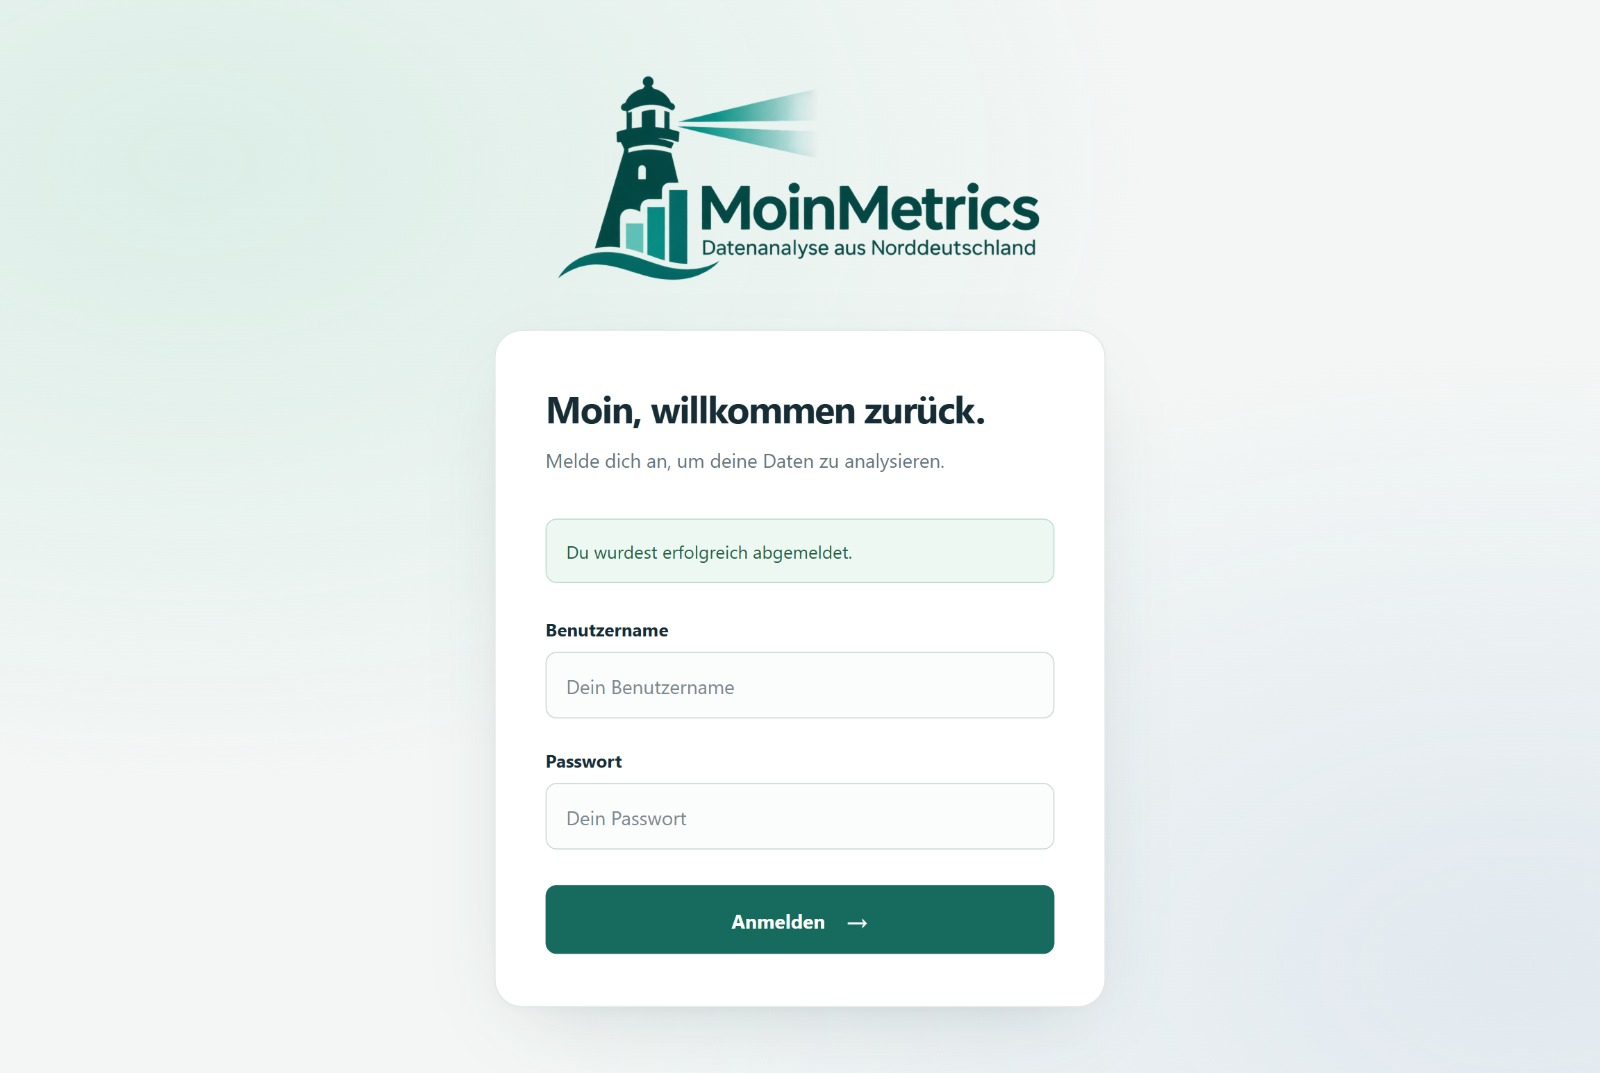
\includegraphics[width=\linewidth]{../screenshot_login.jpeg}
        \caption{Login-Bereich}
    \end{subfigure}\hfill
    \begin{subfigure}[t]{0.48\textwidth}
        \centering
        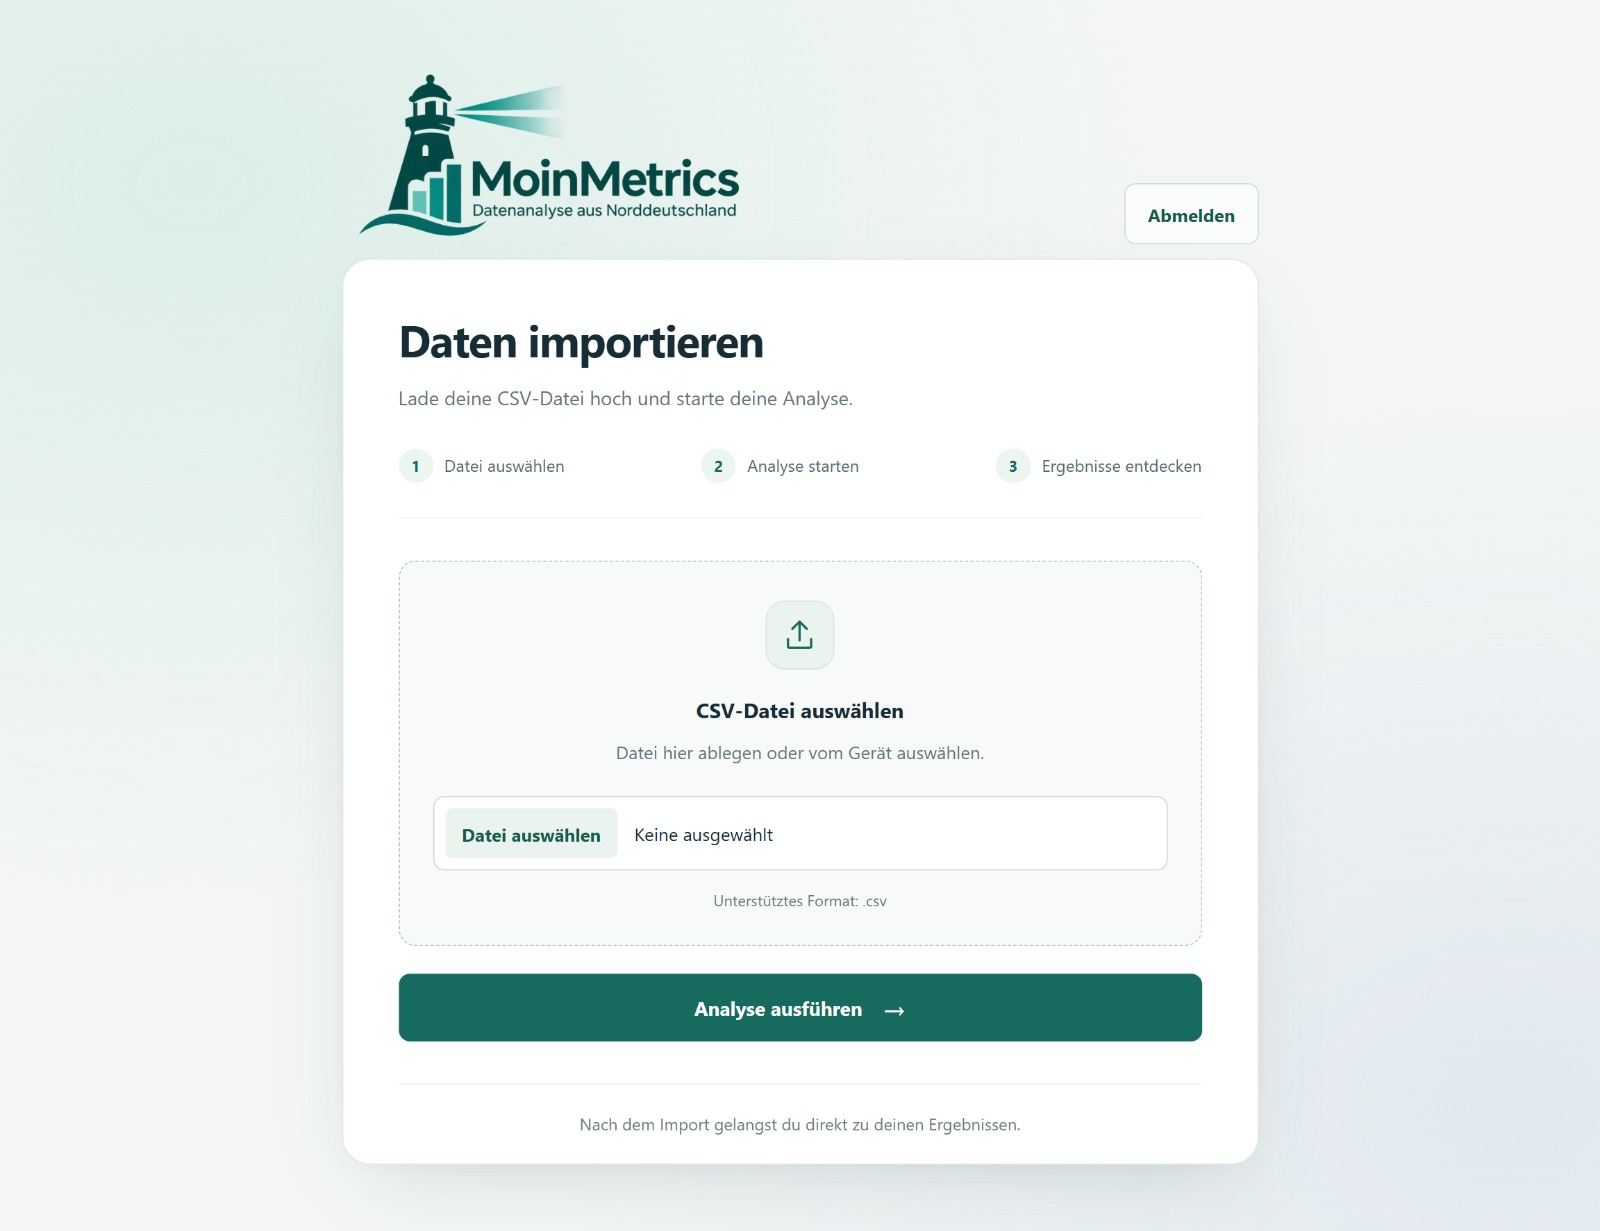
\includegraphics[width=\linewidth]{../screenshot_upload.jpeg}
        \caption{CSV-Upload und Analysestart}
    \end{subfigure}
    \caption{Geschützter Zugang und Upload im Prototyp.}
    \label{fig:login-upload}
\end{figure}

\subsection*{Analyseergebnis auf der Webseite}
Die kompakte Ergebnisansicht fasst zentrale Befunde des Datensatzes zusammen: umsatz- und kundenstarke Wochentage und Uhrzeiten, Top- und Flop-Artikel nach Umsatz und Deckungsbeitrag sowie häufig gemeinsam gekaufte Waren. Der lange Screenshot ist zur besseren Lesbarkeit in zwei aufeinanderfolgende Ausschnitte geteilt.

\begin{figure}[H]
    \centering
    \begin{subfigure}[t]{0.48\textwidth}
        \centering
        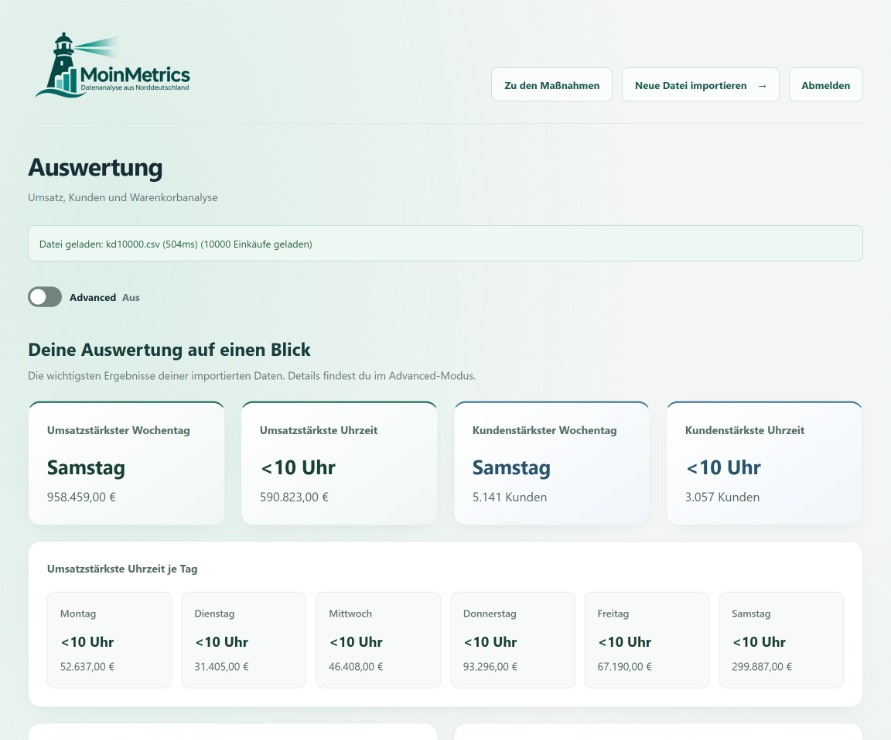
\includegraphics[width=\linewidth]{crops/auswertung_1.jpeg}
        \caption{Kennzahlen und Tagesverläufe}
    \end{subfigure}\hfill
    \begin{subfigure}[t]{0.48\textwidth}
        \centering
        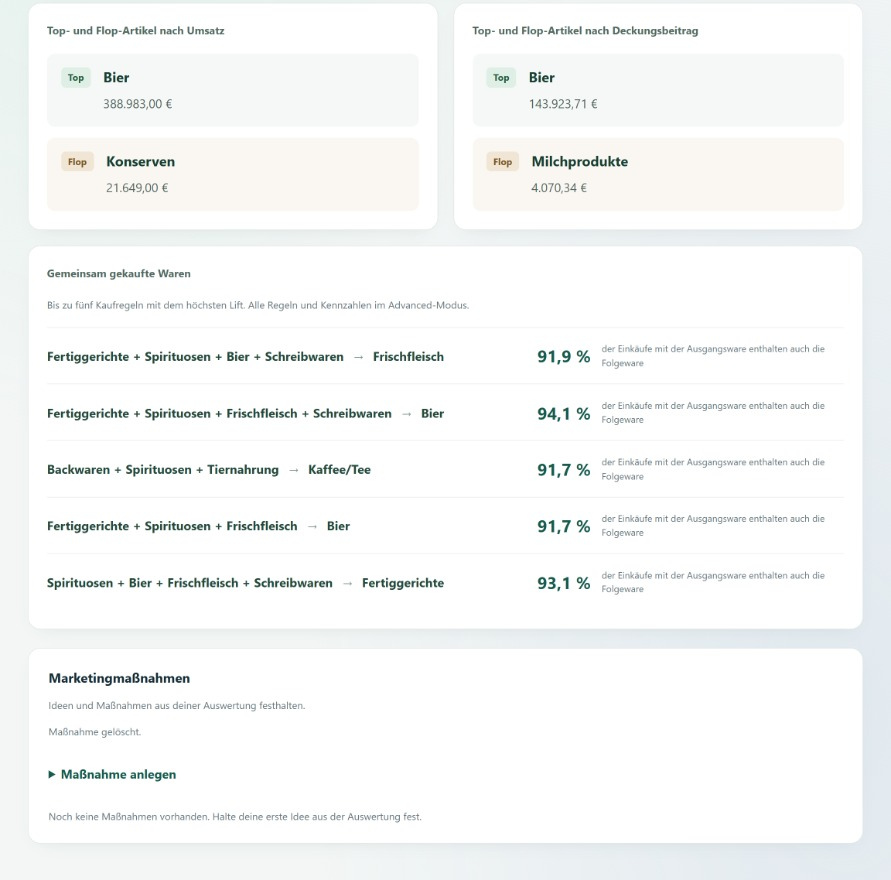
\includegraphics[width=\linewidth]{crops/auswertung_2.jpeg}
        \caption{Artikel, Warenkorbbeziehungen und Maßnahmen}
    \end{subfigure}
    \caption{Kompakte Ergebnisübersicht in zwei aufeinanderfolgenden Ausschnitten.}
    \label{fig:auswertung}
\end{figure}

\clearpage
\subsection*{Erweiterte grafische Darstellung}
Die erweiterte Ansicht ergänzt die kompakte Übersicht um Detailauswertungen. Umsatz und Kundenhäufigkeit werden getrennt dargestellt; weitere Bereiche zeigen Artikelkennzahlen, Warenkorbbeziehungen und Heatmaps. Der lange Screenshot ist in drei aufeinanderfolgende Ausschnitte geteilt, die von links nach rechts gelesen werden.

\begin{figure}[H]
    \centering
    \begin{subfigure}[t]{0.31\textwidth}
        \centering
        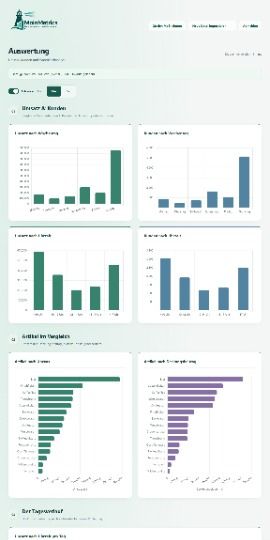
\includegraphics[width=\linewidth]{crops/detail_1.jpeg}
        \caption{Kennzahlen und Artikel}
    \end{subfigure}\hfill
    \begin{subfigure}[t]{0.31\textwidth}
        \centering
        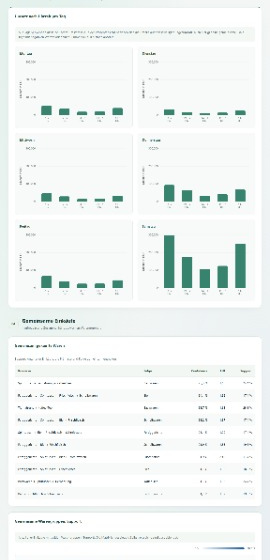
\includegraphics[width=\linewidth]{crops/detail_2.jpeg}
        \caption{Tagesverläufe und Warenkorbbeziehungen}
    \end{subfigure}\hfill
    \begin{subfigure}[t]{0.31\textwidth}
        \centering
        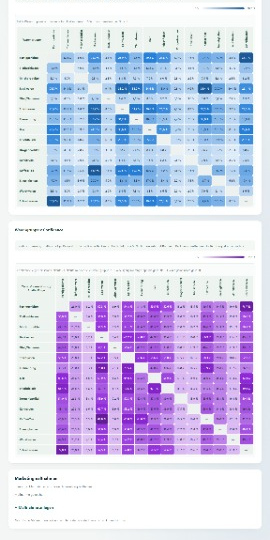
\includegraphics[width=\linewidth]{crops/detail_3.jpeg}
        \caption{Heatmaps und Maßnahmen}
    \end{subfigure}
    \caption{Erweiterte Analyseansicht in drei aufeinanderfolgenden Ausschnitten.}
    \label{fig:metric-ausgabe}
\end{figure}

Die Detailansicht ermöglicht den Vergleich der Kennzahlen. Umsatzsummen und Kundenhäufigkeit bleiben als unterschiedliche Größen erkennbar. Sämtliche angezeigten Werte beziehen sich auf die jeweils importierten Daten.

Zusammen mit der kompakten Übersicht bildet diese Ansicht die Ergebnisstufe des Durchstichs: Der CSV-Import stößt die Analyse an, anschließend werden die berechneten Kennzahlen in der Weboberfläche ausgegeben.
\end{document}
